\begin{itemize*}
	\item Black-box testing:
	\begin{itemize*}
		\item Equivalence partitioning
		\item Boundary value analysis
		\item Error guessing
	\end{itemize*}
	\item White-box testing
	\begin{itemize*}
		\item Statement coverage
		\item Decision / branch coverage
	\end{itemize*}
	\item Black-box and white-box test case design in combination
	\item Basics: heuristics and experience
\end{itemize*}

\begin{figure}
	\centering
	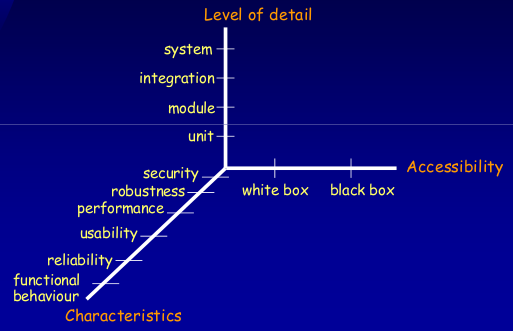
\includegraphics[scale=0.4]{TypesOfTesting}
	\caption Types of Testing
\end{figure}

Development of test cases

\begin{center}
Complete testing is in general impossible\\ $\Rightarrow$\\
Testing cannot guarantee the absence of faults\\ $\Rightarrow$\\
How to select subset of test cases from all possible test cases with a high chance of detecting most faults?\\
$\Rightarrow$\\
Test Case Design Strategies\\
~\\
Because: if we have good test suite then we can have more confidence in the product that passes that test suite
\end{center}

\subsection{Black-Box testing}

\subsubsection{Equivalence Partitioning}

Divide all possible inputs into classes (partitions) such that:
\begin{itemize*}
	\item There is a finite number of input equivalence classes
	\item You may reasonably assume that
	\begin{itemize*}
		\item the program behaves analogously for inputs in the same class
		\item one test with a representative value from a class is sufficient
		\item if the representative detects a fault
		then other class members would detect the same fault
	\end{itemize*}
\end{itemize*}

\begin{figure}[h!]
	\centering
	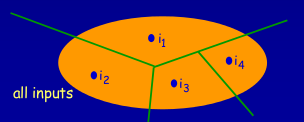
\includegraphics[scale=0.4]{equivalence_partitioning}
\end{figure}

Strategy:
\begin{itemize*}
	\item Identify input equivalence classes
	\begin{itemize*}
		\item Based on conditions on inputs/outputs in specification/description
		\item Both valid and invalid input equivalence classes
		\item Based on heuristics and experience:
		\begin{itemize*}
			\item ``input x in [1..10]''
			$\rightarrow$ classes: x $<$ 1, 1 $\leq$ x $\leq$ 10, x $>$ 10
			\item ``enumeration A, B, C'' $\rightarrow$ classes: A, B, C, not \{A,B,C,\}
			\item ``input integer n''
			$\rightarrow$ classes: n not an integer,
			n $<$ min, min $\leq$ n$<$0, 0$\leq$ n $\leq$max, n $>$max
			\item$\ldots$
		\end{itemize*}
	\end{itemize*}
	\item Define one/couple of test cases for each class
	\begin{itemize*}
		\item Test cases that cover valid classes
		\item Test cases that cover at most one invalid class
	\end{itemize*}
\end{itemize*}

%TODO add example

\subsubsection{Boundary Value Analysis}

Based on experience / heuristics:
\begin{itemize*}
\item Testing boundary conditions of eq. classes is more effective i.e. values directly on, above, and beneath edges of classes
\item Choose input boundary values as tests in input classes instead of, or additional to arbitrary values
\item Choose also inputs that invoke output boundary values (values on the boundary of output classes)
\item Example strategy as extension of equivalence partitioning:
\begin{itemize*}
	\item choose one (n) arbitrary value(s) in each eq. class
	\item choose values exactly on lower and upper boundaries of eq. class
	\item choose values immediately below and above each boundary (if applicable)
\end{itemize*}
\end{itemize*}

%TODO example

\subsubsection{Error Guessing}

\begin{itemize*}
	\item Just `guess’ where the errors are$\ldots$
	\item Intuition and experience of tester
	\item Ad hoc, not really a technique
	\item But can be quite effective
	\item Strategy:
	\begin{itemize*}
		\item Make a list of possible errors or error-prone situations (often related to boundary conditions)
		\item Write test cases based on this list
	\end{itemize*}
	\item More sophisticated `error guessing': Risk Analysis
	\item Try to identify critical parts of program
	(high risk code sections):
	\begin{itemize*}
		\item parts with unclear specifications
		\item developed by junior programmer while his wife was pregnant $\ldots\ldots$
		\item complex code :
		measure code complexity - tools available (McGabe, Logiscope,$\ldots$)
	\end{itemize*}
	\item High-risk code will be more thoroughly tested (or be rewritten immediately $\ldots\ldots$)
	
\end{itemize*}

\subsubsection{Which one?}

\begin{itemize*}
	\item Black-box testing techniques:
	\begin{itemize*}
		\item Equivalence partitioning
		\item Boundary value analysis
		\item Cause-effect graphing
		\item Decision tables
		\item State transition testing
		\item Error guessing
		\item ............
		\begin{itemize*}
			\item test derivation from formal specification
		\end{itemize*}		
	\end{itemize*}
	\item Which one to use?
	\begin{itemize*}
		\item None of them is complete
		\item All are based on some kind of heuristics
		\item They are complementary
	\end{itemize*}
	\item Always use a combination of techniques
	\begin{itemize*}
		\item When a formal specification is available try to use it
		\item Identify valid and invalid input equivalence classes
		\item Identify output equivalence classes
		\item Apply boundary value analysis on valid equivalence classes
		\item Guess about possible errors
		\item Cause-effect graphing for linking inputs and outputs
	\end{itemize*}
\end{itemize*}

\subsection{White-Box Testing}

\begin{itemize*}
	\item Testing based on program code\\
	hence, programming language dependent
	\item Extent to which (source) code is executed, i.e.\ covered
	\item Different kind of coverage:
	\begin{itemize*}
		\item path coverage
		\item statement coverage
		\item (multiple-) condition coverage
		\item decision/branch coverage
		\item $\ldots$
	\end{itemize*}
\end{itemize*}

\subsubsection{Path Testing}

\begin{itemize*}
	\item Execute every possible path of a program, i.e., every possible sequence of statements
	\item Strongest white-box criterion
	\item Usually impossible: infinitely many paths (in case of loops)
	\item So: not a realistic option
	\item But note: enormous reduction w.r.t.\ all possible test cases (each sequence of statements executed for only one value)
\end{itemize*}

%TODO add example

\subsubsection{Statement Coverage}

\begin{itemize*}
	\item Execute every statement of a program
	\item Relatively weak criterion
	\item Weakest white-box criterion
\end{itemize*}

%TODO add example

\subsubsection{Branch Coverage}

\begin{itemize*}
	\item Branch coverage == decision coverage
	\item Execute every branch of a program: each possible outcome of each decision occurs at least once
	\item Example:
	\begin{itemize*}
		\item \verb|IF b THEN s1 ELSE s2|
		\item \verb|CASE x OF|
		\begin{enumerate}
			\item $\ldots$
			\item $\ldots$
			\item $\ldots$
		\end{enumerate}
	\end{itemize*}
\end{itemize*}

%TODO add example

\subsubsection{Condition Coverage}

\begin{itemize*}
	\item Design test cases such that each possible outcome of each condition in each decision occurs at least once
	\item Example:
	\begin{itemize*}
		\item decision (i $<$ N) AND (result $\leq$ maxint) consists of two conditions: (i $<$ value) and (result $\leq$ maxint) test cases should be designed such that each gets value
		true and false at least once
	\end{itemize*}
\end{itemize*}

%TODO add example

\subsubsection{How to apply?}

\begin{itemize*}
	\item Don't start with designing white-box test cases!
	\item Start with black-box test cases
	(equivalence partitioning, boundary value analysis, cause effect graphing, derivation with formal methods, .....)
	\item Check white-box coverage (statement-, branch-, condition-, ...... coverage)
	\item Use a coverage tool
	\item Design additional white-box test cases for not covered code
\end{itemize*}


